% Revised VE Simulation Report
% Arseniy Khvorov
% Created 2019/06/04
% Last edit 2019/06/04

\documentclass[11pt]{article}

\usepackage[utf8x]{inputenc}

%%% PAGE DIMENSIONS
\usepackage{geometry}
\geometry{a4paper}
\geometry{margin=1in} % for example, change the margins to 2 inches all round

\usepackage{graphicx} % support the \includegraphics command and options

\usepackage[parfill]{parskip} % Begin paragraphs with an empty line rather than an indent

%%% PACKAGES
\usepackage{booktabs} % for much better looking tables
\usepackage{array} % for better arrays (eg matrices) in maths
\usepackage{paralist} % very flexible & customisable lists (eg. enumerate/itemize, etc.)
\usepackage{verbatim} % adds environment for commenting out blocks of text & for better verbatim
\usepackage{subfig} % make it possible to include more than one captioned figure/table in a single float
\usepackage{float}

\usepackage[numbers]{natbib}
\bibliographystyle{vancouver}


\usepackage{multicol}
\usepackage{multirow}
\usepackage{xcolor}
\usepackage{amsmath}

\usepackage[T1]{fontenc}
\usepackage{lmodern}

%%% FLOWCHART
\usepackage{tikz} % flowcharts
\usetikzlibrary{shapes.geometric, arrows, positioning, backgrounds}


\renewcommand{\arraystretch}{1.1}

%%% HEADERS & FOOTERS
\usepackage{fancyhdr} % This should be set AFTER setting up the page geometry
\pagestyle{fancy} % options: empty , plain , fancy
\renewcommand{\headrulewidth}{0pt} % customise the layout...
\lhead{\leftmark}\chead{}\rhead{\rightmark}
\lfoot{}\cfoot{\thepage}\rfoot{}

%%% SECTION TITLE APPEARANCE
\usepackage{sectsty}
\allsectionsfont{\sffamily\mdseries\upshape} % (See the fntguide.pdf for font help)
% (This matches ConTeXt defaults)

%%% ToC (table of contents) APPEARANCE
\usepackage[nottoc,notlof,notlot]{tocbibind} % Put the bibliography in the ToC
\usepackage[titles,subfigure]{tocloft} % Alter the style of the Table of Contents
\renewcommand{\cftsecfont}{\rmfamily\mdseries\upshape}
\renewcommand{\cftsecpagefont}{\rmfamily\mdseries\upshape} % No bold!

\usepackage[bookmarks,hidelinks]{hyperref}

%%% END Article customizations

%%% The "real" document content comes below...

\title{VE estimates with administrative data}
\author{Arseniy Khvorov}
\date{October 2019} 

\begin{document}
\maketitle

\renewcommand{\abstractname}{}
\begin{abstract}
	\begin{center}
	Simulation repository\\
	https://github.com/khvorov45/ve-admin
	\end{center}
\end{abstract}

\tableofcontents

\pagebreak

%
\section{Methods}

%%
\subsection{Core simulation}

Starting population was the general population. Its size was set to 500,000. Every individual had their attributes randomly allocated in the order shown in Figure \ref{SimDiag} and with probabilities shown in tables below.

First allocated attribute was true vaccination status. Measurement of this status for the purposes of the simulated study was allowed to be inaccurate in order to simulate exposure miscalssification. True vaccination status was used to determine which probability to use to allocate individuals to the flu-infected category. Both vaccinated and unvaccinated subjects were allocated to the non-flu infected category with the same probability. The remaining subjects ended up as part of the non-ARI category.

Everyone with an ARI (either infected with flu or a non-flu pathogen) was assigned to either the symptomatic or the asymptomatic group. Those who were symptomatic were assigned to the clinically assessed or unassessed groups. Being clinically assessed in this context means that they presented to a clinic with ARI illness and they were classified as an ARI case. These clinically assessed ARI cases got one probability of being tested, everyone else got another. Tests were allowed to be imperfect to simulate outcome misclassification.

%%
\subsection{Population summary}

Each population was collapsed down to summary results - each individual was considered to be part of one of eight categories: administrative/surveillance vaccinated/unvaccinated case/control as shown in Figure \ref{PopAgg}.

\begin{figure}[h]
	\centering
		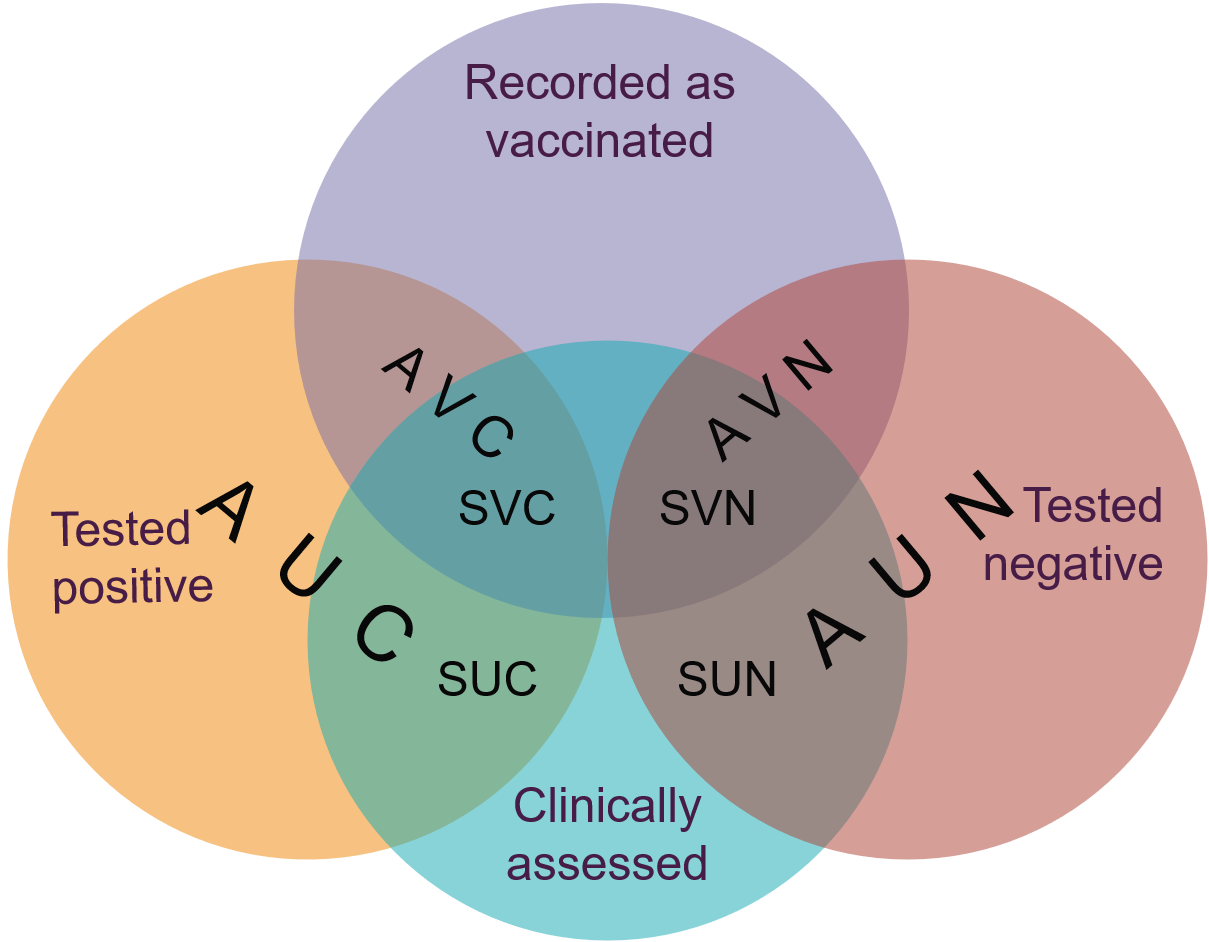
\includegraphics[width=0.5\linewidth]{../sim-diag/popagg-venn.png}
		\caption{
Assignment of an individual to appropriate categories. A - administrative, S - surveillance, V - vaccinated, U - unvaccinated, C - case, N - non-case (control). \label{PopAgg}
		}
\end{figure}

Individuals in each of the categories were counted. These counts were representative of those that could have been obtained if a test-negative study was done on that population either using administrative or surveillance data. VE estimates could then be calculated as 1 - OR where OR = $\frac{\text{Odds in vaccinated}}{\text{Odds in unvaccinated}}$ where Odds = $\frac{\text{Count of cases}}{\text{Count of controls}}$.

\pagebreak

\begin{figure}[H]
	\centering
		\tikzstyle{group} = [rectangle, minimum width=3cm, minimum height=1cm, text centered, text width=3cm, draw=black, fill=black, text=white, fill opacity=0.9, text opacity=1]

\tikzstyle{arrowlab} = [rectangle, fill=black, text=white, fill opacity = 0.9]

\tikzstyle{arrow} = [thick, ->, >=stealth]

\pgfdeclarelayer{bg}
\pgfsetlayers{bg, main}

\begin{tikzpicture}[node distance=2cm]
\node (pop) [group] {Population};
\node (truevac) [group, below of=pop, left of=pop] {True vaccinated};
\node (trueunvac) [group, below of=pop, right of=pop] {True unvaccinated};
\node (recvac) [group, below of=truevac] {Recorded as vaccinated};
\node (recunvac) [group, below of=trueunvac] {Recorded as unvaccinated};
\node (nonflu) [group, below of=recunvac, left of=recunvac] {Non-flu};
\node (nonari) [group, below left=1cm and 1cm of nonflu] {Non-ARI};
\node (flu) [group, right=1cm of nonflu] {Flu};
\node (ari) [group, below of=flu, left of=flu] {ARI};
\node (sympt) [group, below of=ari] {Symptomatic};
\node (asympt) [group, left=1cm of sympt] {Asymptomatic};
\node (clin) [group, below of=sympt] {Clinically assessed};
\node (nonclin) [group, left=1cm of clin] {Unassessed};
\node (test) [group, below of=clin] {Tested};
\node (nontest) [group, left=1cm of test] {Not tested};
\node (fluinf) [group, below of=test] {Flu-infected};
\node (notfluinf) [group, left=1cm of fluinf] {Non flu-infected and uninfected};
\node (pos) [group, below of=fluinf] {Positive};
\node (neg) [group, left=1cm of pos] {Negative};

\draw[arrow] (pop) -- node[arrowlab] {$v$} (truevac);
\draw[arrow, dashed] (pop) -- (trueunvac);

\draw[arrow] (truevac) -- node[arrowlab] {$s_{e,v}$} (recvac);
\draw[arrow, dashed] (truevac) -- (recunvac);
\draw[arrow] (trueunvac) -- node[arrowlab] {$s_{p,v}$} (recunvac);
\draw[arrow, dashed] (trueunvac) -- (recvac);

\begin{pgfonlayer}{bg}
\draw[arrow] (truevac) -- node[arrowlab, yshift=-1cm, xshift=1.5cm] {$f(1-e)$} (flu);
\draw[arrow] (truevac) -- node[arrowlab, yshift=-1cm, xshift=0.5cm] {$l$} (nonflu);
\draw[arrow] (trueunvac) -- node[arrowlab, yshift=-1cm, xshift=0.75cm] {$f$} (flu);
\draw[arrow] (trueunvac) -- node[arrowlab, yshift=-1cm, xshift=-0.5cm] {$l$} (nonflu);
\draw[arrow, dashed] (trueunvac) -- (nonari);
\draw[arrow, dashed] (truevac) -- (nonari);

\draw[arrow, dotted] (nonari) -- (nonclin);
\end{pgfonlayer}

\draw[arrow, dotted] (nonflu) -- (ari);
\draw[arrow, dotted] (flu) -- (ari);

\draw[arrow] (ari) -- node[arrowlab] {$p$} (sympt);
\draw[arrow, dashed] (ari) -- (asympt);

\draw[arrow] (sympt) -- node[arrowlab] {$c$} (clin);
\draw[arrow, dashed] (sympt) -- (nonclin);

\draw[arrow, dotted] (asympt) -- (nonclin);

\draw[arrow] (clin) -- node[arrowlab] {$t_a$} (test);
\draw[arrow, dashed] (clin) -- (nontest);
\draw[arrow] (nonclin) -- node[arrowlab, yshift=-0.2cm, xshift=0.5cm] {$t_n$} (test);
\draw[arrow, dashed] (nonclin) -- (nontest);

\draw[arrow] (test) -- (fluinf);
\draw[arrow, dashed] (test) -- (notfluinf);

\draw[arrow] (fluinf) -- node[arrowlab] {$s_e$} (pos);
\draw[arrow, dashed] (fluinf) -- (neg);
\draw[arrow] (notfluinf) -- node[arrowlab] {$s_p$} (neg);

\end{tikzpicture}
		\caption{
Simulation decision tree. Parameter key is in Table \ref{TabParKey}. Solid lines mean allocation with probabilities represented by the indicated parameters. Dashed line probabilities are complements of corresponding solid line probabilities. Dotted lines represent full-group allocation. Probability of being flu-infected for those who are tested isn't indicated because it wasn't necessary for the purposes of simulations. \label{SimDiag}
		}
\end{figure}

\pagebreak
%%
\subsection{Parameter Variation}

Every parameter in the simulation was set at a prespecified value. Some of the parameters were set to vary (their prespecified value would have been ignored then). Setting a parameter to vary meant meant that the parameter was assigned a small set of values, set to the first of those values, a set amount of populations were simulated using that value, then it was set to the next value and so on until the simulation went through the entire set.

If multiple parameters were set to vary the simulation would have gone through all possible combinations of all parameters values.

%%
\subsection{Mixed-group simulations}

If a simulation required a population to be composed of multiple groups, each group was simulated as if it were a separate population. The only mixed combination used was children/adults/elderly. The total size of each group was obtained by multiplying the total requested sample size (usually 200,000) by the specified proportion of each group in the population (this is the $w$ parameter which would have been set to 1 if there was only one group in the population). Amounts of cases and controls were counted in each of the groups and added together to represent the counts obtained from the full population.

%%
\subsection{Additional simulations}

To determine the effects of individual parameters, an additional set of simulations was performed with parameters fixed to values shown in Table \ref{AddSim}. This set of parameter values produced unbiased VE estimates in surveillance data. Using this as a baseline, required parameters could be varied (e.g. $s_p$ can be set below 1) to observe their effect in absence of other sources of bias. Additional simulations were also used to observe the effect some parameters have on others (e.g. how $s_p$ set below 1 affects variation of VE estimates at different values of $t_n$).

\pagebreak
%%
\subsection{Parameter estimates used}

\begin{table}[h]
\centering
\caption{
Parameter names, meanings and values used in simulations. "Range used" shows the range of values used for variation in individual age group simulations. Tables \ref{TabComb} contains values and patterns used for variation in mixed group simulations. Every parameter except $c$ represents an absolute probability (some of them only apply to subsets of the population). Only relative probability estimates could be obtained for $c$ (by comparing presentation counts found in ASPREN data \cite{ASPREN} to expected underlying population size derived from other parameter estimates), its values were  set to 1 in individual group simulations unless it is the parameter varied. Parameter $w$ was only relevant if the population was requested to be composed of multiple groups. Shown values are the ones used in children/adults/elderly mixed simulation. In individual simulations, $w$ was set to 1. Estimates of $v$ and $e$ were derived from provided data. \label{TabParKey}
}
	% Table generated by Excel2LaTeX from sheet 'ParEstUsedInd'
\begin{tabular}{cp{13.285em}>{\centering}p{4.57em}cccc}
\toprule
\textnormal{Par.} & \multicolumn{1}{c}{Description} & Range Used & \multicolumn{1}{p{4.215em}}{Children (<15)} & \multicolumn{1}{p{4.07em}}{Adults (15-65)} & \multicolumn{1}{p{3.5em}}{Elderly (65+)} & Ref. \\
\midrule
$w$  & Proportion of the age groups in the general population &  & 0.189 & 0.657 & 0.154 & \cite{ABSDemo} \\
$v$ & Probability of being vaccinated & 0.05 - 0.5 & 0.1  & 0.25  & 0.66 &  \\
$s_{e,v}$ & Sensitivity of exposure measurement & 0.9 - 1 & 0.9  & 0.95  & 0.98 & \cite{Irving;2009, Donald;1999, Rolnick;2013} \\
$s_{p,v}$ & Specificity of exposure measurement & 0.5 - 1 & 0.9  & 0.8  & 0.7 & \cite{Irving;2009, Donald;1999, Rolnick;2013} \\
$e$    & Vaccine effectiveness & 0.1 - 0.9 & 0.6  & 0.5  & 0.4 & \\
$f$ & Influenza risk in unvaccinated & 0.05 - 0.15 & 0.15  & 0.08  & 0.05 & \cite{Tokars;2017} \\
$l$ & Non-influenza ARI risk in vaccinated and unvaccinated & 0.1 - 0.3 & 0.3   & 0.15  & 0.1 & \cite{ADH2017, ADH2018} \\
$p$ & Probability of the ARI being symptomatic & 0.1 - 0.9 & 0.84  & 0.84  & 0.84 & \cite{Leung;2015} \\
$c$ & Relative probability of being clinically assessed as having ARI when it is symptomatic & 0.1 - 0.9 & 0.4 & 0.3 & 1 & \\
$t_a$ & Tested probability for clinically assessed ARI & 0.1 - 0.9 & 0.17  & 0.35  & 0.22 & \cite{ASPREN} \\
$t_n$ & Tested probability for everyone without clinically assessed ARI & 0 - 0.3 & 0.15  & 0.15  & 0.15 & \\
$s_e$ & Sensitivity of influenza test & 0.5 - 1 & 0.86  & 0.86  & 0.86 & \cite{Druce;2004} \\
$s_p$ & Specificity of influenza test & 0.9 - 1 & 0.984 & 0.984 & 0.984 & \cite{Druce;2004} \\
\bottomrule
\end{tabular}%

\end{table}

\pagebreak

\begin{table}[h]
\centering
\small
\caption{
Combinations (patterns of variation) and values used in fixed variation of parameters when multiple groups were present in the population. Combinations 1 and 3 were not used for $w$. \label{TabComb}
}
	% Table generated by Excel2LaTeX from sheet 'ParEstUsedMultPat'
\begin{tabular}[t]{rccc}
\toprule
\multicolumn{1}{c}{Combination} & Children & Adults & Elderly \\
\midrule
1     & Low   & Low   & Low \\
2     & Mid   & Mid   & Mid \\
3     & High  & High  & High \\
4     & High  & Low   & Low \\
5     & Low   & High  & Low \\
6     & Low   & Low   & High \\
\bottomrule
\end{tabular}%
 \quad
	% Table generated by Excel2LaTeX from sheet 'ParEstUsedMultVals'
\begin{tabular}[t]{>{\ttfamily}c<{\normalfont}ccc}
\toprule
\textnormal{Parameter} & Low   & Mid   & High \\
\midrule
$w$  & 0.15  & 0.33  & 0.7 \\
$v$ & 0.05  & 0.3   & 0.5 \\
$s_{e,v}$ & 0.9   & 0.95  & 1 \\
$s_{p,v}$ & 0.5   & 0.75  & 1 \\
$e$    & 0.1   & 0.5   & 0.9 \\
$f$ & 0.05  & 0.1   & 0.15 \\
$l$ & 0.1   & 0.15  & 0.3 \\
$p$ & 0.1   & 0.5   & 0.9 \\
$c$ & 0.1   & 0.5   & 0.9 \\
$t_a$ & 0.1   & 0.5   & 0.9 \\
$t_n$ & 0     & 0.15  & 0.3 \\
$s_e$ & 0.5   & 0.75  & 1 \\
$s_p$ & 0.9   & 0.95  & 1 \\
\bottomrule
\end{tabular}%

\end{table}

\begin{table}[h]
\centering
\small
\caption{
Parameter values used in the additional simulation set. Parameter $w$ is missing because the additional simulations were always performed with only one parameter set in the population (equivalent to only having one age group). \label{AddSim}
}
	% Table generated by Excel2LaTeX from sheet 'SpecialPopulations'
\begin{tabular}[t]{lc}
\toprule
Parameter & Value \\
\midrule
$v$ & 0.5 \\
$s_{e,v}$ & 1 \\
$s_{p,v}$ & 1 \\
$e$     & 0.5 \\
$f$  & 0.3 \\
$l$  & 0.3 \\
$p$ & 1 \\
$c$ & 1 \\
$t_a$ & 1 \\
$t_n$ & 1 \\
$s_e$ & 1 \\
$s_p$ & 1 \\
\bottomrule
\end{tabular}%

\end{table}

\pagebreak
%
\section{Results and discussion}

The following sections present and discuss results associated with every parameter whose variation within ranges defined in Table \ref{TabParKey} had a perceivable effect on the bias of VE estimates.

%%
\subsection{Individual-group simulations}

%%
\subsubsection{Effect of tested proportions --- $t_a$ and $t_n$}

Changing $t_a$ (test probability for those with clinically assessed ARI) and $t_n$ (test probability for everyone else) only affected the estimates of VE in administrative data as shown in Figures \ref{agesind-ta} and \ref{agesind-tn} respectively. The parameter that allowed the pattern seen in Figure \ref{agesind-ta} to be replicated in the additional simulation set was influenza test specificity $s_p$ when set below 1. No additional simulation replicated the pattern seen in Figure \ref{agesind-tn} (most obvious in the elderly group).

\begin{figure}[H]
	\centering
		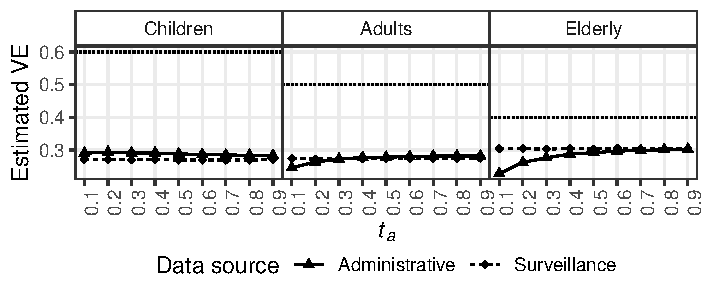
\includegraphics[width=.75\linewidth]{../fig-agesind/agesind-test_clin.pdf}
		\caption{
Effect of changing $t_a$ in different populations. All groups were simulated individually. The dotted line is the true value. \label{agesind-ta}
		}
		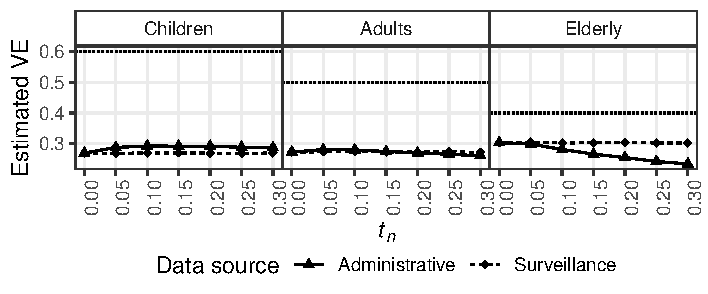
\includegraphics[width=.75\linewidth]{../fig-agesind/agesind-test_nonclin.pdf}
		\caption{
Effect of changing $t_n$ in different populations. All were simulated inidvidually. The dotted line is the true value. \label{agesind-tn}
		}
\end{figure}

\pagebreak

The reason why only administrative data is affected is the fact that when $t_a$ changed, $t_n$ remained fixed and vice versa. As $t_a$ decreased, administrative sample became more and more different from surveillance due to there being a decreasing proportion of people with ARI in the population who get tested and a constant proportion without ARI who get tested. This compositional difference can also be created by fixing $t_a$ and increasing $t_n$. The results produced are equivalent - as the administrative sample becomes more compositionally different from the surveillance sample, the administrative estimate bias may increase. 

The reason why no additional simulation replicated the pattern in Figure \ref{agesind-tn} is likely the fact that additional simulations only allowed one parameter other than $t_n$ to introduce bias. The pattern seen is likely a result of multiple parameters other than $t_n$ introducing bias. Hence no additional simulation set had enough ``accumulated'' bias to replicate the pattern closely.

%%
\subsubsection{Effect of true vaccine effectiveness ($e$)}

Variation of the parameter affected both surveillance and administrative estimates of VE --- they were more biased with higher true VE values, especially so in children as shown in Figure \ref{agesind-ve}.

\begin{figure}[h]
	\centering
		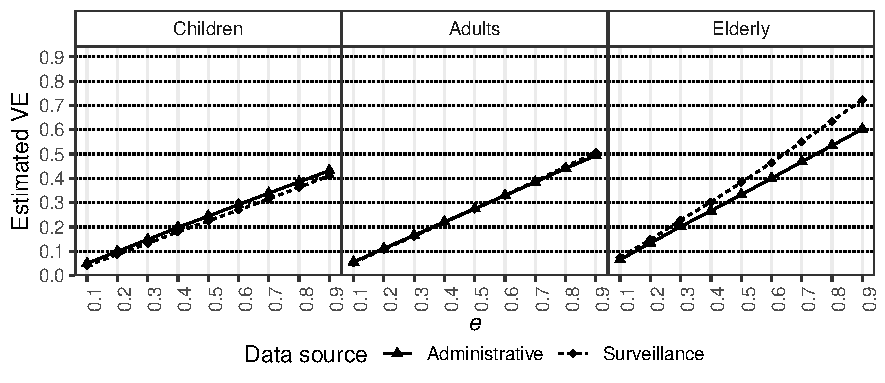
\includegraphics[width=0.75\linewidth]{../fig-agesind/agesind-ve.pdf}
		\caption{
Effect of changing $e$ in different populations. All were simulated inidvidually. The dotted line is the true value. \label{agesind-ve}
		}
\end{figure}

The parameter responsible for the greater bias in children was most likely the vaccinated proportion $v$ as children had it set to the lowest value of the three groups. Since the additional simulations that had low $v$ did not have the pattern replicated, it is likely that low $v$ increases bias at high $e$ only in presence of misclassification. This was confirmed when more simulations were run where $e$ and $v$ were both varied in different misclassification settings. Results in Figure \ref{veinv-summ} showed that the pattern is only replicated with low $v$ and non-one $s_{p,v}$.

\pagebreak

\begin{figure}[H]
	\centering
		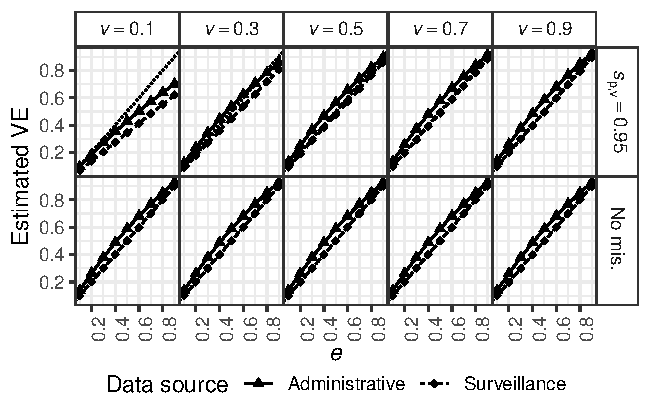
\includegraphics[width=0.85\linewidth]{../fig-veinv/veinv-limited.pdf}
		\caption{
Effect of changing both $e$ and $v$ while also allowing for misclassification. The other parameters were set to values shown in Table \ref{AddSim} . Only miscalssification setting shown is decreased $s_{p,v}$. Other settings (decreased $s_{e,v}$,  $s_p$, $s_e$) produced results similar to those of no miscalssificaiton. \label{veinv-summ}
		}	
\end{figure}

The fact that in absence of miscalssification neither vaccine effectiveness nor vaccinated proportion will be expected to have an effect on the bias of a test-negative odds ratio can be shown in Table \ref{tab:veinv1} and Eq.\ \ref{eq:veinv1}.

\begin{table}[h]
\centering
\caption{
Expected proportions of surveillance data.
Assumptions: no misclassification, $t_a$= 1, $t_n$= 1.
$F$ - flu-infected, $V$ - vaccinated.
 \label{tab:veinv1}
}
	\begin{tabular}{ccc}
\toprule
 & $F$ & $\bar{F}$ \\
\midrule
$V$ & $vf(1-e)$ & $vl$ \\
$\bar{V}$ & $(1-v)f_u$ & $(1-v)l$ \\
\bottomrule
\end{tabular}
\end{table}

\begin{equation} \label{eq:veinv1}
OR = 1-e
\end{equation}

When misclassification is added in a form of imperfect specificity of vaccination status measurement, bias is introduced as seen in Table \ref{tab:veinv2} and Eq.\ \ref{eq:veinv2}

\begin{table}[h]
\centering
\caption{
Expected proportions of surveillance data. Assumptions: no misclassification other than $s_{p,v}$, $t_a$= 1,$t_n$= 1.
$F$ - flu-infected, $V$ - vaccinated
 \label{tab:veinv2}
}
	\begin{tabular}{ccc}
\toprule
 & $F$ & $\bar{F}$ \\
\midrule
$V$ & $vf(1-e)+(1-s_{p_v})(1-v)f$ & $vl + (1-s_{p,v})(1-v)l$ \\
$\bar{V}$ & $(1-v)fs_{p,v}$ & $(1-v)ls_{p,v}$ \\
\bottomrule
\end{tabular}
\end{table}

\begin{equation} \label{eq:veinv2}
\begin{aligned}
OR &= \frac{v(1-e)+(1-s_{p,v})(1-v)}{v+(1-s_{p,v})(1-v)} =  \frac{v-ev+1-s_{p,v}-v+s_{p,v}v}{v+1-v-s_{p,v}+s_{p,v}v} =  
	\frac{s_{p,v}v-s_{p,v}-ev+1}{s_{p,v}v-s_{p,v}+1} \\
	&= \frac{s_{p,v}(v-1)+1-ev}{s_{p,v}(v-1)+1} = 1 - \frac{ev}{s_{p,v}(v-1)+1}
\end{aligned}
\end{equation}

This OR will approach the unbiased $1-e$ as $v$ increases. Eq.\ \ref{eq:veinv3} shows that the bias will increase with $e$ but only if $s_{p,v}<1$. When $s_{p,v}=1$ the bias is 0.

\begin{equation} \label{eq:veinv3}
\begin{aligned}
B &= OR_{\text{biased}} - RR_{\text{true}} = 1 - \frac{ev}{s_{p,v}(v-1)+1} - (1-e) = e - \frac{ev}{s_{p,v}(v-1)+1} \\
	&= e(1 - \frac{v}{s_{p,v}(v-1)+1})
\end{aligned}
\end{equation}

For a given value of $e$, the bias is proportional to $1 - \frac{v}{s_{p,v}(v-1)+1}$ meaning that it depends on $v$ but only if $s_{p,v}<1$. When $s_{p,v}=1$ the bias is 0.

The overall effect of true VE is such that as long as there is imperfect vaccination status measurement specificity, higher values of it will result in greater bias and this bias will be affected by vaccinated proportion - the smaller the proportion the greater the bias. 

Other misclassification types can allow true VE to introduce bias as well but simulation results showed that it would not be as prominent as the one discussed above (associated with $s_{p,v}$), and it would not depend on vaccinated proportion which is why it would not explain the differences between age groups in Figure \ref{agesind-ve}. Effect of other types of misclassification will be discussed in their own sections.

Since miscalssification can always be expected, highly efficacious vaccines are likely to be underestimated to a greater degree than less efficacious vaccines, especially so when only a small proportion of the population is vaccinated.

%%
\subsubsection{Effect of specificity of vaccination status measurement ($s_{p,v}$)}

Variation of this parameter affected both surveillance and administrative estimates of VE - they are more biased with at lower values. This effect was most pronounced in children and least so in elderly. The reason for this is the fact that children had the lowest vaccinated proportion. As a result, they had the lowest number of true vaccinated cases and non-cases to which exposure misclassification would add subjects who were truly unvaccinated but classified as vaccinated. Since the true numbers in children were low, this misclassification had a greater impact on VE estimate bias than it did in the other groups.

\pagebreak

\begin{figure}[h]
	\centering
		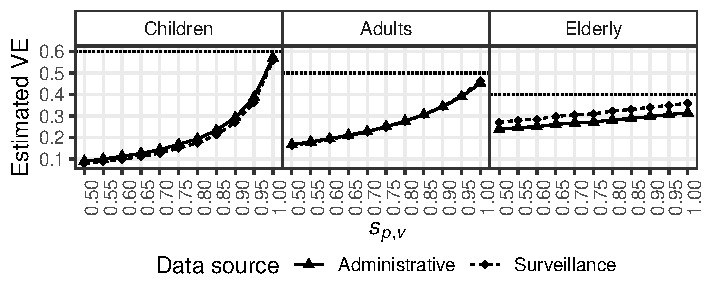
\includegraphics[width=0.75\linewidth]{../fig-agesind/agesind-spec_vac.pdf}
		\caption{
Effect of changing $s_{p,v}$ in different populations. All were simulated inidvidually. The dotted line is the true value. \label{fig:agesind-spv}
		}
\end{figure}

%%
\subsubsection{Effect of influenza test specificity ($s_p$) and influenza incidence ($f$)}

Variation of $s_p$ affected both surveillance and administrative estimates of VE --- they are more biased with at lower values. This effect was most pronounced in administrative data in the elderly as shown in Figure \ref{fig:agesind-spf}.

\begin{figure}[h]
	\centering
		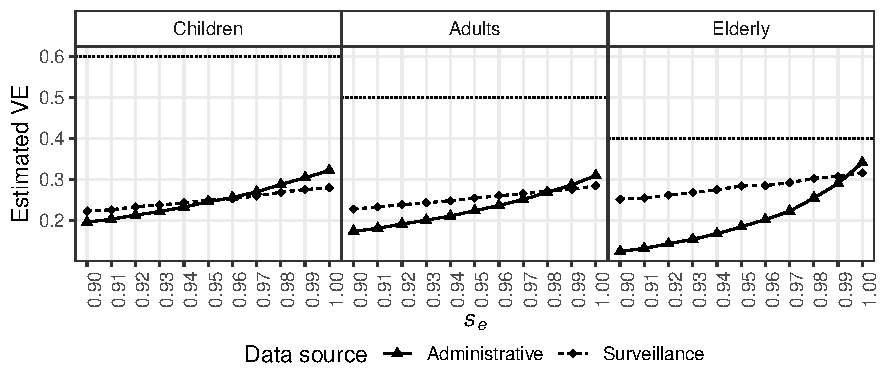
\includegraphics[width=0.75\linewidth]{../fig-agesind/agesind-spec_flu.pdf}
		\caption{
Effect of changing $s_p$ in different populations. All were simulated inidvidually. Dashed line is the true value. \label{fig:agesind-spf}
		}
\end{figure}

Administrative data appears to be more sensitive to outcome misclassification. The effect is most obvious in the elderly due to them having the lowest $f$. To show this, the expected proportions are shown in Table \ref{SFexplanationMath}. Eq. \ref{EqSFORA} and \ref{EqSFORAll} show expected ORs in surveillance and administrative data. Figure \ref{SFIPfGraph} graphs both equations at various values of $s_p$ and $f$.

\pagebreak

\begin{table}[h]
\centering
\caption{
Expected proportions in a population. Shown for ARI and non-ARI subjects separately. Surveillance sample would only contain ARI subjects, administrative would contain everyone. $T_p$ - tested as flu-infected, $T_n$ - tested as uninfected $V$ - vaccinated, $A$ - ARI.
Assumptions: no misclassification other than $s_p$, $t_a$= 1, $t_n$= 1
\label{SFexplanationMath} 
}
	\begin{tabular}{ccccc}
\toprule
 &\multicolumn{2}{c}{$T_p$} & \multicolumn{2}{c}{$T_n$}  \\
 & $A$ & $\bar{A}$ & $A$ & $\bar{A}$  \\
\midrule
$V$ & $vf(1-e)+vl(1-s_p)$ & $v(1-s_p)(1-l-f(1-e))$ & $vls_p$ & $vs_p(1-l-f(1-e))$ \\
$\bar{V}$ & $(1-v)f+(1-v)l(1-s_p)$ & $(1-v)(1-s_p)(1-l-f)$ & $(1-v)ls_p$ & $(1-v)s_p(1-l-f)$ \\
\bottomrule
\end{tabular}
\end{table}

\begin{equation} \label{EqSFORA}
OR_{\text{surveillance}} = \frac{f(1-e)+l(1-s)}{f+l(1-s)}
\end{equation}

\begin{equation} \label{EqSFORAll}
OR_{\text{administrative}} = \frac{\Big(1-s(1-f(1-e))\Big)\Big(s(1-f)\Big)}{\Big(1-s(1-f)\Big)\Big(s(1-f(1-e))\Big)}
\end{equation}

\begin{figure}[h]
	\centering
		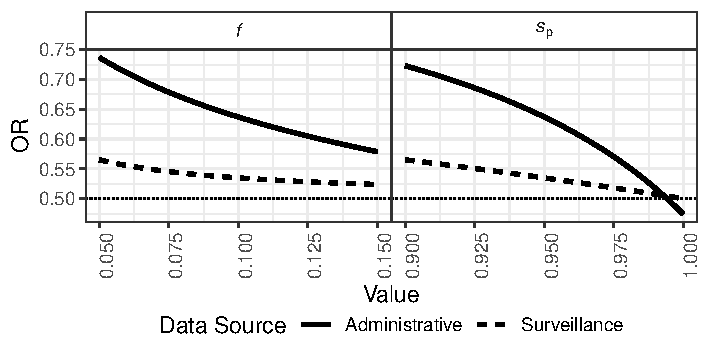
\includegraphics[width=0.75\linewidth]{../fig-sfinv/sfinv.pdf}
		\caption{
The impact of flu incidence and specificity. $s_p$ was graphed at $f$ of 0.1; $f$ was graphed at $s_p$ of 0.95. Both had true VE ($e$) set to 0.5 and $l$ to 0.15. \label{SFIPfGraph}
		}
\end{figure}

It can be seen from the figure that  decrease in either parameter leads to bias towards the null (1). Additionally, administrative data is affected to a greater extent than surveillance. This agrees with the simulations where $s_p$ was seen to affect administrative data more so than surveillance and the greatest impact was seen in elderly who had the lowest $f$.

The biasing effect of high $f$ can be seen as a result of violating the rare disease assumption. In absence of miscalssification this would introduce bias away from the null in administrative data while surveillance data would remain unbiased. However, administrative data also appears to be more susceptible to outcome miscalssification. So at any value of $f$ in absence of miscalssification, administrative data will be biased away from the null, while in presence of outcome misclassification (particularly imperfect specificity) it will be more biased towards the null due to its higher susceptibility to miscalssification. This can be seen in the cross-over of lines in the $s_p$ panel of Figure \ref{SFIPfGraph}.

\pagebreak

%%
\subsubsection{Effect of sensitivities ($s_{e,v}$ and $s_e$)}
%%

Variation of these parameters within the plausible range had little effect of both surveillance and administrative estimates in every group --- they are slightly more biased with at lower values as shown in Figures \ref{agesind-sev} and \ref{agesind-spv}.

\begin{figure}[h]
	\centering
		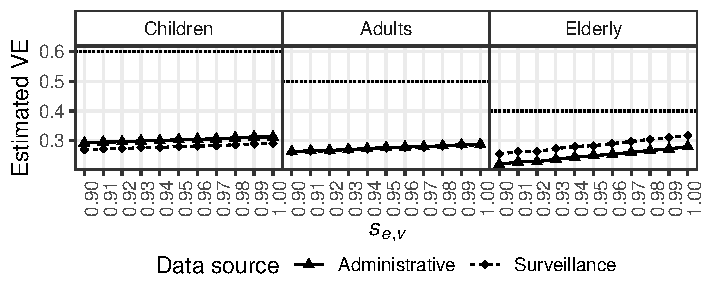
\includegraphics[width=0.75\linewidth]{../fig-agesind/agesind-sens_vac.pdf}
		\caption{
Effect of changing $s_{e,v}$ in different populations. All were simulated inidvidually. The dotted line is the true value. \label{agesind-sev}
		}
		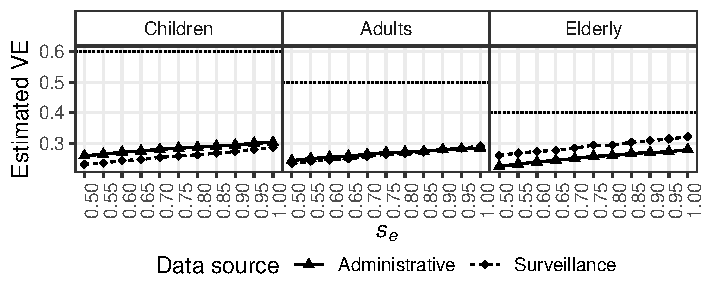
\includegraphics[width=0.75\linewidth]{../fig-agesind/agesind-sens_flu.pdf}
		\caption{
Effect of changing $s_e$ in different populations. All were simulated inidvidually. The dotted line is the true value. \label{agesind-spv}
		}
\end{figure}

\pagebreak
%
\subsection{Mixed-group simulations}

Bias is generally negative (towards the null). Administrative data is generally more biased in the same direction as surveillance.

\subsubsection{Effect of $t_n$}

Under certain conditions, the overall administrative VE estimate can become much more biased than the overall surveillance estimate or any of the group-specific estimates. This happened in the simulations when$t_n$ was set to a high value (0.3) either in the elderly or in children and to a low value (0) in the other groups as shown in Figure \ref{agesmult-tn}

\begin{figure}[h]
	\centering
		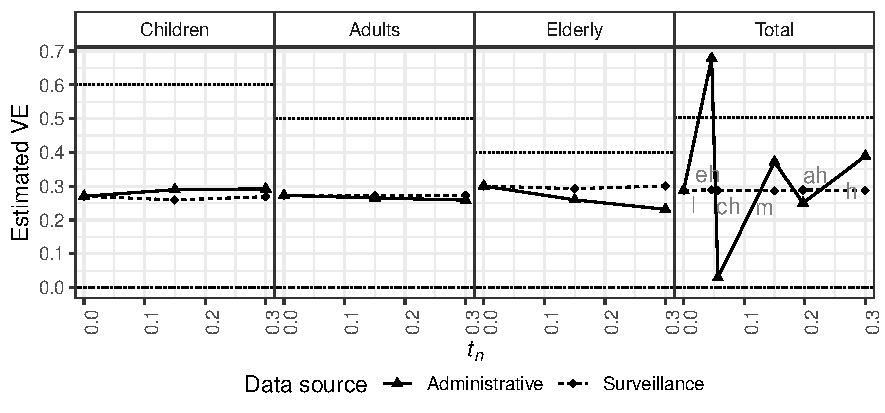
\includegraphics[width=1\linewidth]{../fig-agesmult/agesmult-test_nonclin.pdf}
		\caption{
Effect of changing $t_n$ in a population with multiple groups. Dashed line is the true value. Dotted line is drawn at VE estimate of 0. The three panels on the left show group-specific VE estimates. The right-most panel shows the VE estimates calculated from the whole sample ignoring age. Letters correspond to parameter combinations shown in Table \ref{TabComb}: all low (l), all mid (m), all high (h), children low (cl), adults low (al), elderly low (el). The overall administrative estimate under is more biased when $t_n$ is set to a high value in the elderly or in the children than under other combinations. \label{agesmult-tn}
		}
\end{figure}

The results above show that when $t_n$ changes among groups, the overall unadjusted estimate of VE of administrative data can swing in either direction.

The reason for this is that those who do not have an ARI but are included into the study will mostly contribute to the study's non-cases. If the majority of the ARI-free people are vaccinated, then their contribution to vaccinated controls will be greater than to vaccinated cases. This only becomes a problem for the odds ratio (and vaccine effectiveness) estimates when the groups are mixed and the estimates are coming from the overall population.

To illustrate, let's say there is a population with 3 age subgroups and non-ARI individuals are only tested in one of them. Table \ref{TabExCntIndividual} shows expected counts and odds ratio (OR).

\begin{table}[h]
\centering
\caption{
Expected proportions of administrative data in a population with three age groups. $h_v = 1 - (1-e)f - l$ represents the probability of staying healthy for a vaccinated individual. $h_u = 1 - f - l$ represents the probability of staying healthy for an unvaccinated individual.
Assumptions: no misclassification, $t_a=1$, $t_n=1$ in group 1 and 0 otherwise, disease incidence is the same in all groups, all groups have the same size. 
 \label{TabExCntIndividual}
}
	\begin{tabular}{cp{5em}p{5em}p{5em}cc}
\toprule
Group & Cases vaccinated & Cases unvaccinated & Controls vaccinated & Controls unvaccinated & OR \\
\midrule
1 & $v_1(1-e)f$ & $(1-v_1)f$ & $v_1(l+h_v)$ & $(1-v_1)(l+h_u)$ & $\frac{(1-e)(l+h_u)}{(l+h_v)}$ \\
2 & $v_2(1-e)f$ & $(1-v_2)f$ & $v_2l$ & $(1-v_2)l$ & $1-e$ \\
3 & $v_3(1-e)f$ & $(1-v_3)f$ & $v_3l$ & $(1-v_3)l$ & $1-e$ \\
\bottomrule
\end{tabular}
\end{table}

If the OR were to be calculated for individual age subgroups, it would be unbiased if they only contain people with ARI (groups 2 and 3). Some bias is introduced with "contamination" by healthy people. This corresponds to a traditional case-control study - control subjects are selected from everyone who isn't a case (as opposed to everyone with an ARI who isn't a case). With low flu incidence $h_u \simeq h_v$ so the bias is small. 

The overall population is where bias has the potential to swing in a more pronounced manner. Table \ref{TabExCntOverall} shows expected counts in the overall population (made up of subgroups 1, 2 and 3) for both surveillance and administrative data.

\begin{table}[h]
\centering
\caption{
Expected proportions in the overall population. The first row is a population made up of the three age groups in Table \ref{TabExCntIndividual}. The second row is the counts we would have gotten if the first subgroup in Table \ref{TabExCntIndividual} did not have healthy people in control groups (i.e. if all groups had $t_n$ set to 0). This corresponds to surveillance data counts. \label{TabExCntOverall}
}
	\begin{tabular}{cp{7em}p{7em}p{6.5em}p{6.5em}c}
\toprule
Data type & Cases vaccinated & Cases unvaccinated & Controls vaccinated & Controls unvaccinated & OR \\
\midrule
Administrative & $(1-e) f \sum_{i=1}^3 v_i$ & $f \sum_{i=1}^3 (1-v_i)$ & $v_1h_v+l \sum_{i=1}^3 v_i$ & $h_u(1-v_1) + l\sum_{i=1}^3(1-v_i)$ & Eq. \ref{ORBad} \\[30pt]
Surveillace & $(1-e)f \sum_{i=1}^3 v_i$ & $f \sum_{i=1}^3 (1-v_i)$ & $l \sum_{i=1}^3 v_i$ & $l\sum_{i=1}^3(1-v_i)$ & $1-e$ \\
\bottomrule
\end{tabular}

\end{table}

Surveillance data would only include those with ARI which is why it is not affected by the "contamination" by healthy people which is experienced by administrative data hence its odds ratio is unbiased. However the OR coming from administrative data would have this form:

\begin{equation} \label{ORBad}
OR_{1 2 3} = \frac
{(1-e) \sum_{i=1}^3 v_i \Big[ h_u(1-v_1) + l\sum_{i=1}^3(1-v_i) \Big]}
{\sum_{i=1}^3 (1-v_i) \Big[ v_1h_v+l \sum_{i=1}^3 v_i \Big]}
\end{equation}

The issue comes from the fact that group 1 can contribute different counts to numerator and denominator and therefore make the OR swing in either direction. Figure \ref{ORbadVGraph} demonstrates how the vaccinated proportion in subgroup 1 can affect the overall OR.

\pagebreak
\thispagestyle{plain}
\bibliography{references}

\end{document}
